\begin{onehalfspace}

Il disegno distingue correttezza ideale dell'aritmetica, comportamento sotto
rumore controllato e capacità del post-processing di utilizzare l'istogramma.
Qui sono fissati perimetro, appaiamento e regole decisionali; i risultati sono
nel Capitolo~\ref{chap:risultati}.

\section{Disegno e perimetro sperimentale}
\label{sec:obiettivi_sperimentali}

La prima fase applica tre strategie allo \emph{stesso} istogramma: M1 verifica
la sola moda (TOP-1), TOP-4 i primi quattro candidati, M2 usa un classificatore
per decidere se attivare la stessa ricerca TOP-4. Quest'ultima è l'ablazione che
separa il contributo del modello da quello della ricerca multi-candidato.

Le campagne rumorose usano $N=15$, $a=7$, con i due preset uniformi della
Tabella~\ref{tab:contratto_n15}, che non simulano la calibrazione di una QPU
specifica. Le istanze ulteriori sono validate soltanto in condizioni ideali;
scelte aritmetiche, costi e perimetro completo sono nella
Sezione~\ref{app:shor_perimetro_esteso}.

\begin{table}[!htbp]
\centering
\small
\caption{Contratto essenziale delle campagne rumorose su $N=15$.}
\label{tab:contratto_n15}
\begin{tabular}{lcc}
\toprule
\textbf{Parametro} & \textbf{Riferimento} & \textbf{Stress} \\
\midrule
$a$ / periodo atteso & $7/4$ & $7/4$ \\
qubit di controllo / shot & $8/1024$ & $8/1024$ \\
$\lambda_{1q}$ / $\lambda_{2q}$ & $10^{-3}/10^{-2}$ & $5\!\times\!10^{-3}/5\!\times\!10^{-2}$ \\
$T_1/T_2$ (ns) & $100\,000/80\,000$ & $50\,000/30\,000$ \\
$p_{\mathrm{ro}}$ & $0.02$ & $0.05$ \\
\bottomrule
\end{tabular}
\end{table}

\subsection{Scelta dell'aritmetica e limite di scala}
\label{sec:scelta_aritmetica}

La sintesi dell'esponenziazione modulare come operatore unitario denso cresce
come $O(4^k)$ su $k$ qubit~\cite{Barenco1995}. Per le istanze oltre il circuito
didattico viene quindi usata l'aritmetica reversibile di
Beauregard~\cite{beauregard2002}, che costruisce nel dominio della \ac{QFT} gli
addizionatori modulari con costo $O(n^3)$ e $2n+3$ qubit. La riduzione
asintotica non elimina il costo concreto: per $N=21$, $a=2$ e otto qubit di
conteggio, la compilazione congiunta in \texttt{rz/sx/x/cx} produce 21\,036
porte \ac{CX} e profondità 23\,081 su 22 qubit.

Per questo la correttezza di $N=21$ viene verificata idealmente mediante truth
table, azzeramento delle ancille e distribuzione della \ac{QPE}, mentre la
campagna rumorosa rimane su $N=15$. Il costo dominante non è la sola
trasformata finale della phase estimation, ma anche le trasformate interne agli
addizionatori: l'esperimento \ac{AQFT} del Capitolo~\ref{chap:risultati} agisce
proprio in quel punto. Questa separazione evita di presentare un limite della
simulazione classica come limite dell'algoritmo quantistico; la derivazione
estesa è nella Sezione~\ref{app:shor_perimetro_esteso}.

\section{Pipeline appaiata}
\label{sec:architettura}

\begin{figure}[!htbp]
\centering
\resizebox{0.94\textwidth}{!}{%
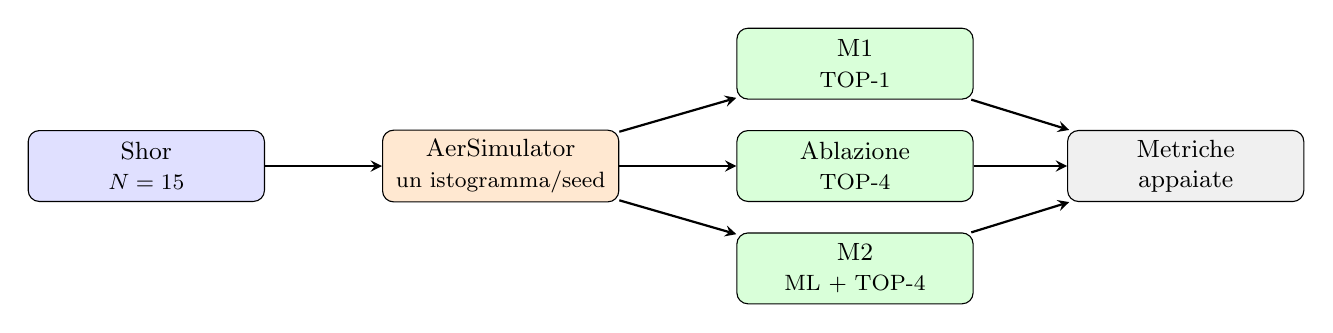
\begin{tikzpicture}[
 box/.style={rectangle,draw,rounded corners=4pt,minimum width=3cm,
             minimum height=0.9cm,align=center,font=\small},
 arrow/.style={->,thick,>=stealth}]
\node[box,fill=blue!12] (shor) at (0,0) {Shor\\{\footnotesize $N=15$}};
\node[box,fill=orange!18] (noise) at (4.5,0) {AerSimulator\\{\footnotesize un istogramma/seed}};
\node[box,fill=green!15] (m1) at (9,1.3) {M1\\{\footnotesize TOP-1}};
\node[box,fill=green!15] (mt4) at (9,0) {Ablazione\\{\footnotesize TOP-4}};
\node[box,fill=green!15] (m2) at (9,-1.3) {M2\\{\footnotesize ML + TOP-4}};
\node[box,fill=gray!12] (out) at (13.2,0) {Metriche\\appaiate};
\draw[arrow] (shor)--(noise);
\draw[arrow] (noise)--(m1); \draw[arrow] (noise)--(mt4); \draw[arrow] (noise)--(m2);
\draw[arrow] (m1)--(out); \draw[arrow] (mt4)--(out); \draw[arrow] (m2)--(out);
\end{tikzpicture}}
\caption{Ogni istogramma è riutilizzato dalle tre strategie: le differenze non
dipendono da realizzazioni Monte Carlo diverse.}
\label{fig:pipeline_architettura}
\end{figure}

Il circuito è compilato una volta nella base \texttt{rz/sx/x/cx}, con livello
di ottimizzazione 2 e seed fissato; la netlist di riferimento ha
224 \texttt{cx} e profondità 412. Per ogni coppia replica--iterazione Aer
produce un istogramma poi condiviso da M1, TOP-4 e M2. Manifest, hash e regola
deterministica per i pareggi sono riportati nella
Sezione~\ref{app:contratto_metodo_esteso}.

\section{Modello di rumore e controlli}
\label{sec:mitigazione_scelte}
\label{subsec:transpilazione}
\label{subsec:noise_uniforme}

Le rotazioni \texttt{rz} sono cambi di frame virtuali. Su \texttt{sx/x} e
\texttt{cx} si compongono depolarizzazione e rilassamento termico, con durate
di 50 e 300\,ns; il readout è una matrice simmetrica. Aer definisce
$\mathcal E(\rho)=(1-\lambda)\rho+\lambda I/2^n$; pertanto, sulle 224 CX,
\begin{equation}
 P_{\mathrm{no\text{-}Pauli\text{-}2Q}}=
 \left(1-\frac{15\lambda}{16}\right)^{224}.
 \label{eq:proxy_no_pauli_2q}
\end{equation}
È un proxy di nessun evento Pauli 2Q, non la probabilità di successo di Shor,
e non comprende errori 1Q, rilassamento o readout.

\label{subsec:readout_mitigation}
Il contratto base non inverte la matrice di readout. $T_1/T_2$, errori 1Q/2Q,
readout, shot, $K$ e ottimizzazione sono variati nelle sensibilità; griglia e
confronto \ac{ZNE} sono nella Sezione~\ref{app:parametrica}.
\label{subsec:zne}
\label{subsec:sensitivity}

\section{Regole decisionali e analisi statistica}
\label{subsec:scelta_ml}
\label{sec:metodo1}
\label{sec:metodo2}

M1 prova un candidato, TOP-4 fino a quattro e M2 gli stessi quattro soltanto se
il classificatore accetta l'istogramma. Dataset, modello TOP-1 e audit TOP-16
sono documentati nella Sezione~\ref{app:classificatore}. Ogni scenario usa 30
repliche, al massimo 50 iterazioni e sentinella 51 per i fallimenti. I confronti
M1$>$TOP-4 e M1$>$M2 impiegano Wilcoxon appaiato unilaterale con
\texttt{zero\_method='pratt'}; TOP-4--M2 è bilaterale. Le correzioni multiple
sono applicate entro la famiglia dichiarata; medie e tassi sono descrittivi,
l'inferenza usa i vettori appaiati completi.

\section{Matrice di verifica dell'intero disegno}

La Tabella~\ref{tab:verifica_requisiti} collega ogni componente alla prova che
la rende controllabile. In questo modo la prima fase, i laboratori QEC, il
surface code, la decodifica, la sensibilità di Shor e l'\ac{AQFT} appartengono
a un solo contratto sperimentale pur mantenendo metriche non intercambiabili.

\begin{table}[!htbp]
\centering
\small
\begin{tabularx}{\textwidth}{@{}p{0.23\textwidth}XX@{}}
\toprule
\textbf{Oggetto} & \textbf{Test o controllo} & \textbf{Evidenza richiesta} \\
\midrule
Circuito $N=15$ & moltiplicatore $\times7\bmod15$, periodo e fattori & truth table, $r=4$, fattori 3 e 5, hash della netlist \\
Aritmetica $N=21$ & azione sui vettori validi e uncomputation & output modulare corretto, ancille a zero e costo compilato \\
M1/TOP-4/M2 & stessi istogrammi, budget e seed & vettori appaiati, Wilcoxon--Pratt e correzione Holm \\
Classificatore & separazione train/validation/test & F1, AUC e audit delle etichette sul test indipendente \\
Ripetizione e Steane & iniezioni correggibili e sweep a piccolo $p$ & sindrome, $\gamma\simeq2$ e regione di break-even \\
Surface code & sweep con distanze crescenti & intervalli su $p_L$ e incrocio compatibile con $p_{th}$ \\
Decoder appreso/ibrido & stessi detection events del \ac{MWPM} & differenza appaiata nei modelli matched e mismatched \\
Shor M8 & sweep del proxy per gate e ripetizioni & curva e $P(k)$, senza conversione dai tassi QEC \\
\ac{AQFT} & sweep della soglia nelle QFT interne & risparmio di porte contro perdita algoritmica \\
\bottomrule
\end{tabularx}
\caption{Corrispondenza fra componenti, controlli e criteri di evidenza.}
\label{tab:verifica_requisiti}
\end{table}

\end{onehalfspace}
